\scanpage{107}

Décomposition en facteurs des fonctions entières.

\margin{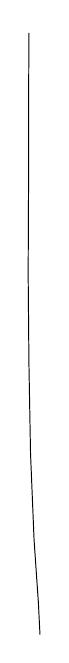
\begin{tikzpicture}[x=0.005cm,y=-0.005cm,baseline={(0,0)}]
\draw[line width=0.35pt] (19,13) -- (18,210) -- (18,400) -- (17,625) -- (19,855) -- (23,1080) -- (32,1300) -- (43,1460) -- (47,1540);
\end{tikzpicture}}
\uline{Théorème 1} (Weierstrass) Soit $f(z)$ fonction entière, $(a_n)$ la suite de ses zéros, rangés par ordre \unsure{en|de} modules croissants. Supposons $f(0)\ne0$. Il est possible de trouver une suite croissante de nombres entiers $\geq0$ $p_n$, et une fonction entière $g(z)$, tels que l'on ait

\[
 f(z)=e^{g(z)}\prod_n\left(1-\frac{z}{a_n}\right)e^{\frac{z}{a_n}+\frac{z^2}{2a_n^2}\unsure{+}\mathord{\cdot}\mathord{\cdot}\frac{z^{p_n}}{p_n a_n^{p_n}}} \tag*{(1)}
\]

le produit étant uniformément absolument convergent quand $z$ parcourt n'importe quelle région bornée. Si \deleted{de plus} \inserted{une suite d'entiers} $p_n$ vérifie

\[
 \sum\left|\frac{r}{a_n}\right|^{(p_n+1)}<+\infty\qquad\text{quel que soit }r,
\]

alors on peut employer cette suite dans l'expression \uline{1}. En particulier, supposons $k$ un entier tel que $\sum\frac{1}{|a_n|^{k+1}}<+\infty$, alors on peut prendre $p_n\deleted{\unsure{=|k}}\unsure{=}p$ pour \deleted{tout} $n$, avec $p\leq k$ d'où

\[
 f(z)=e^{g(z)}\prod_n\left(1-\frac{z}{a_n}\right)e^{\frac{z}{a_n}+\unsure{-|\cdots}+\frac{z^k}{ka_n^k}} \tag*{(2)}
\]

\margin{108}
